% !TEX root = ../../1-te.tex
\tocheck{4}{Aktuelle Musterstudienpläne der FG beschaffen (abängig von der BPO!) und einfügen
}
\label{musterstudienplan}
\iftoggle{winter}{
	\begin{minipage}[H]{1.0\linewidth}
	\begin{center}
		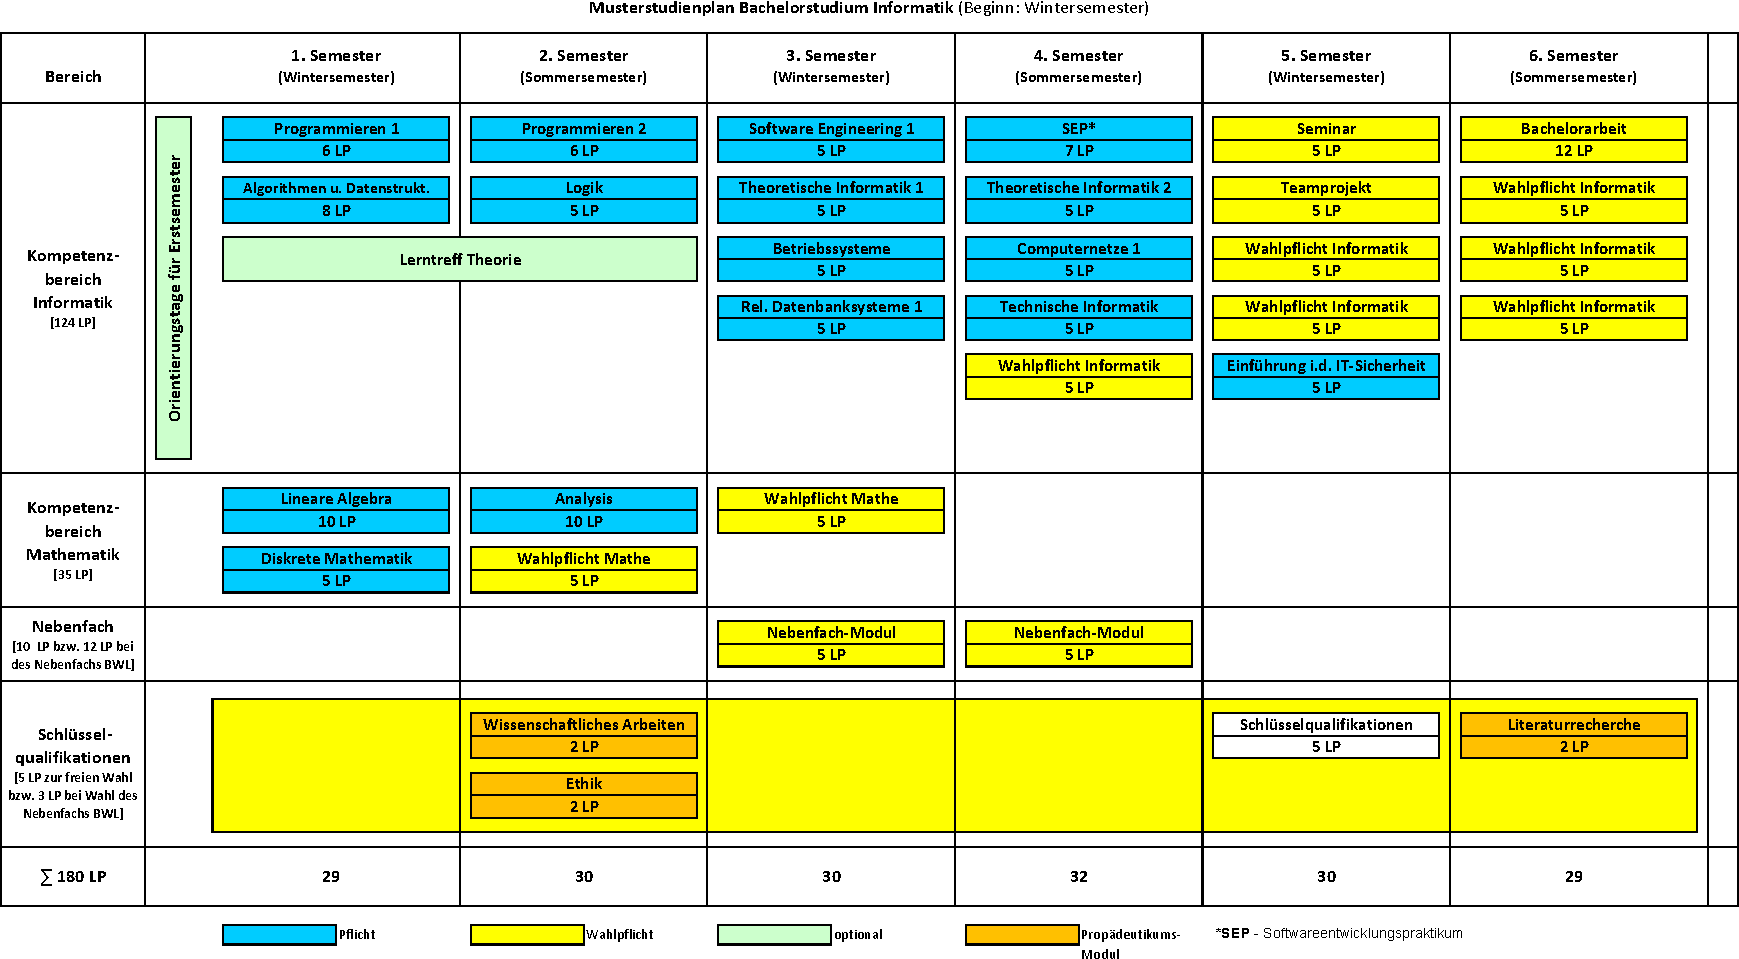
\includegraphics[angle=90, height=\textheight]{bilder/studienplan_bsc/WS-Fak.pdf}
	\end{center}  
	\end{minipage}

	\newpage

	\begin{minipage}[H]{1.0\linewidth}
	\begin{center} 
		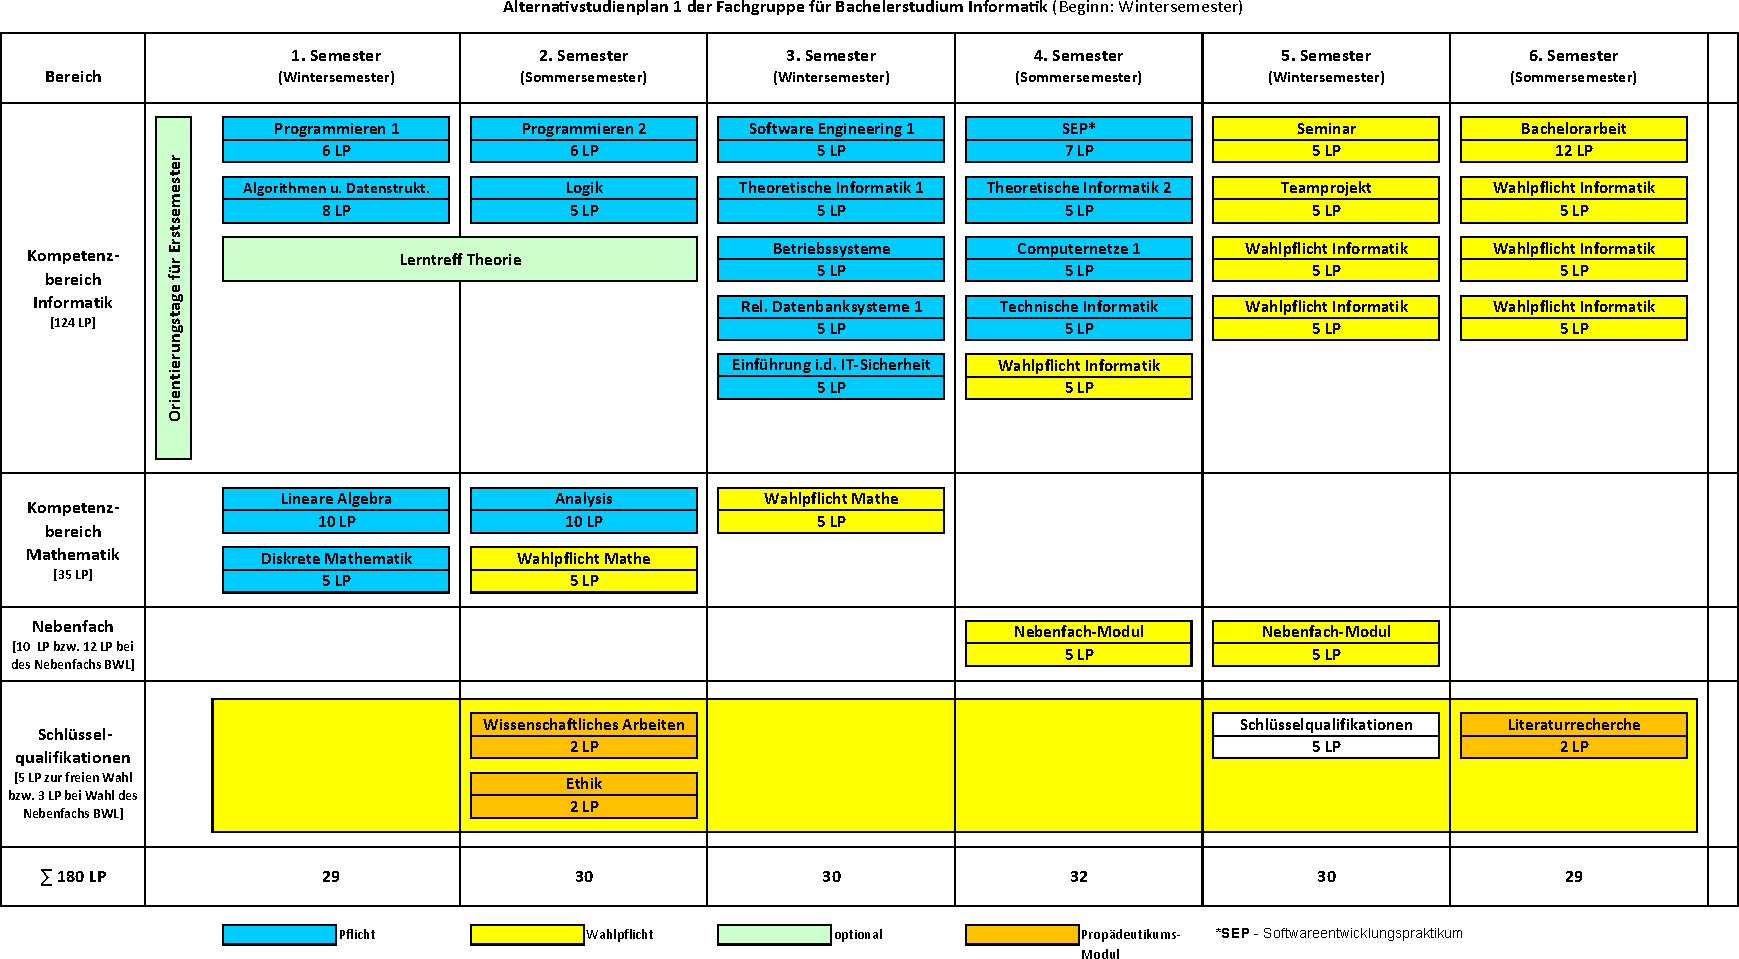
\includegraphics[angle=90, height=\textheight]{bilder/studienplan_bsc/WS-FG-easy.pdf}
	\end{center}
	\end{minipage}

	\newpage

	\begin{minipage}[H]{1.0\linewidth}
	\begin{center} 
		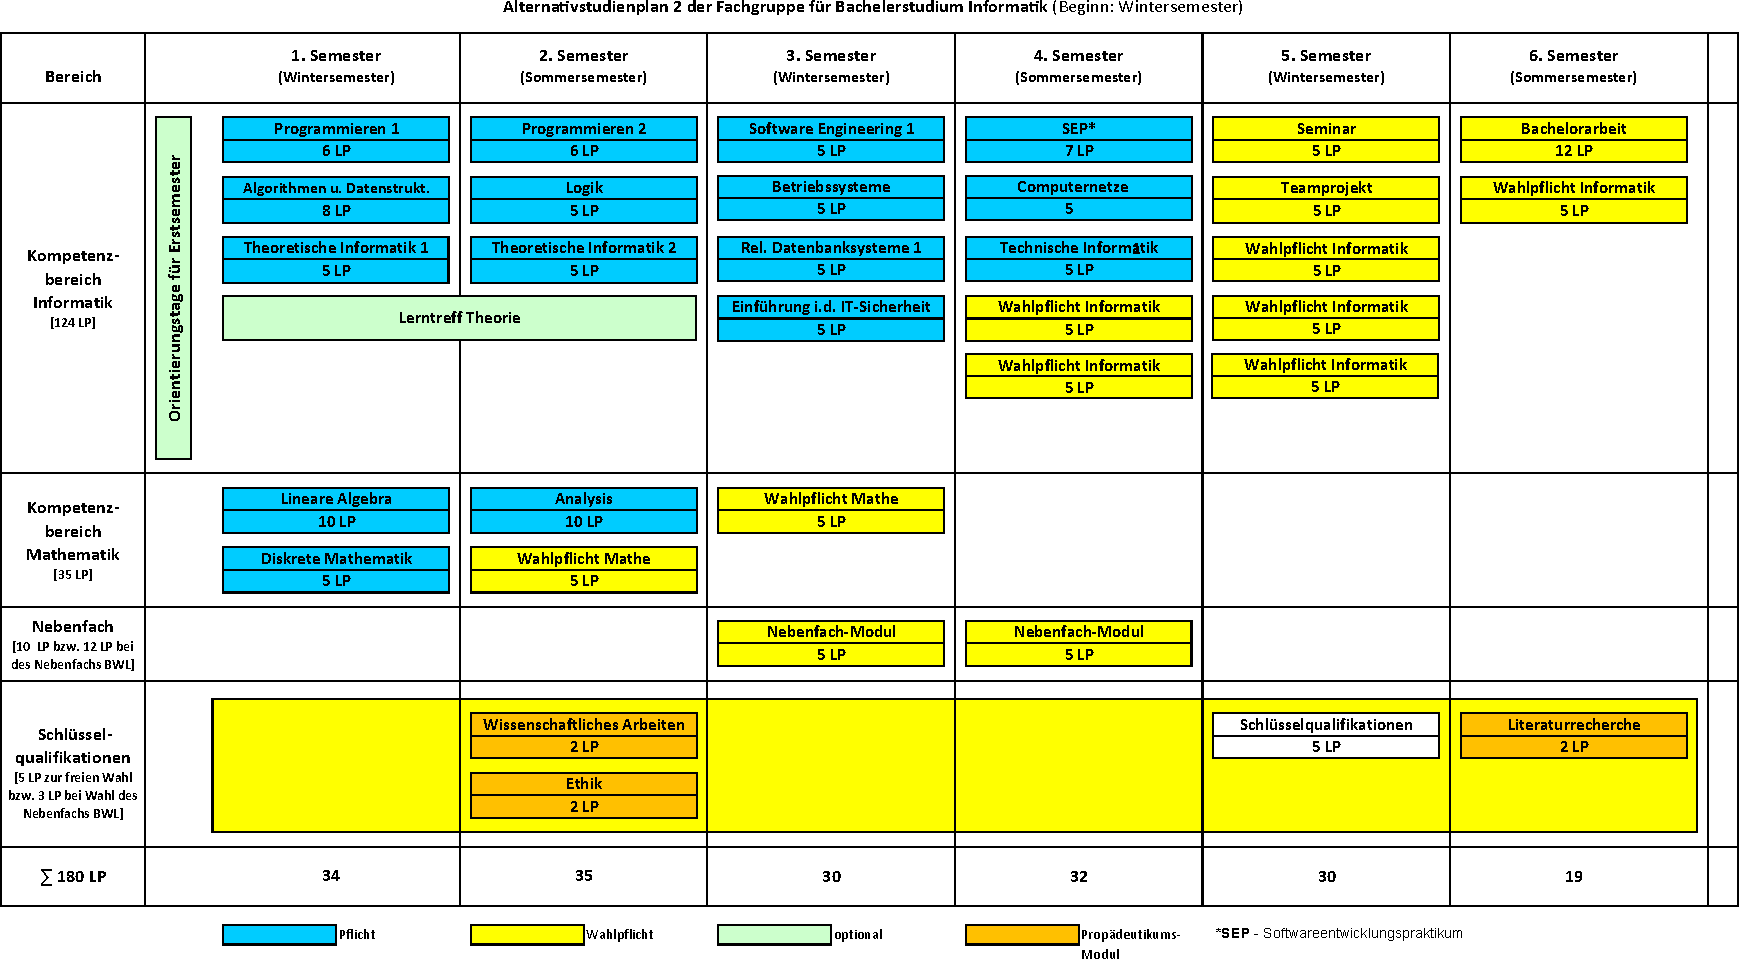
\includegraphics[angle=90, height=\textheight]{bilder/studienplan_bsc/WS-FG-hard.pdf}
	\end{center}
	\end{minipage}
}{
	\tocheck{4}{Aktuelle Musterstudienpläne für SS erzeugen!}

	% \begin{minipage}[H]{1.0\linewidth}
	% 	\begin{center}
	% 	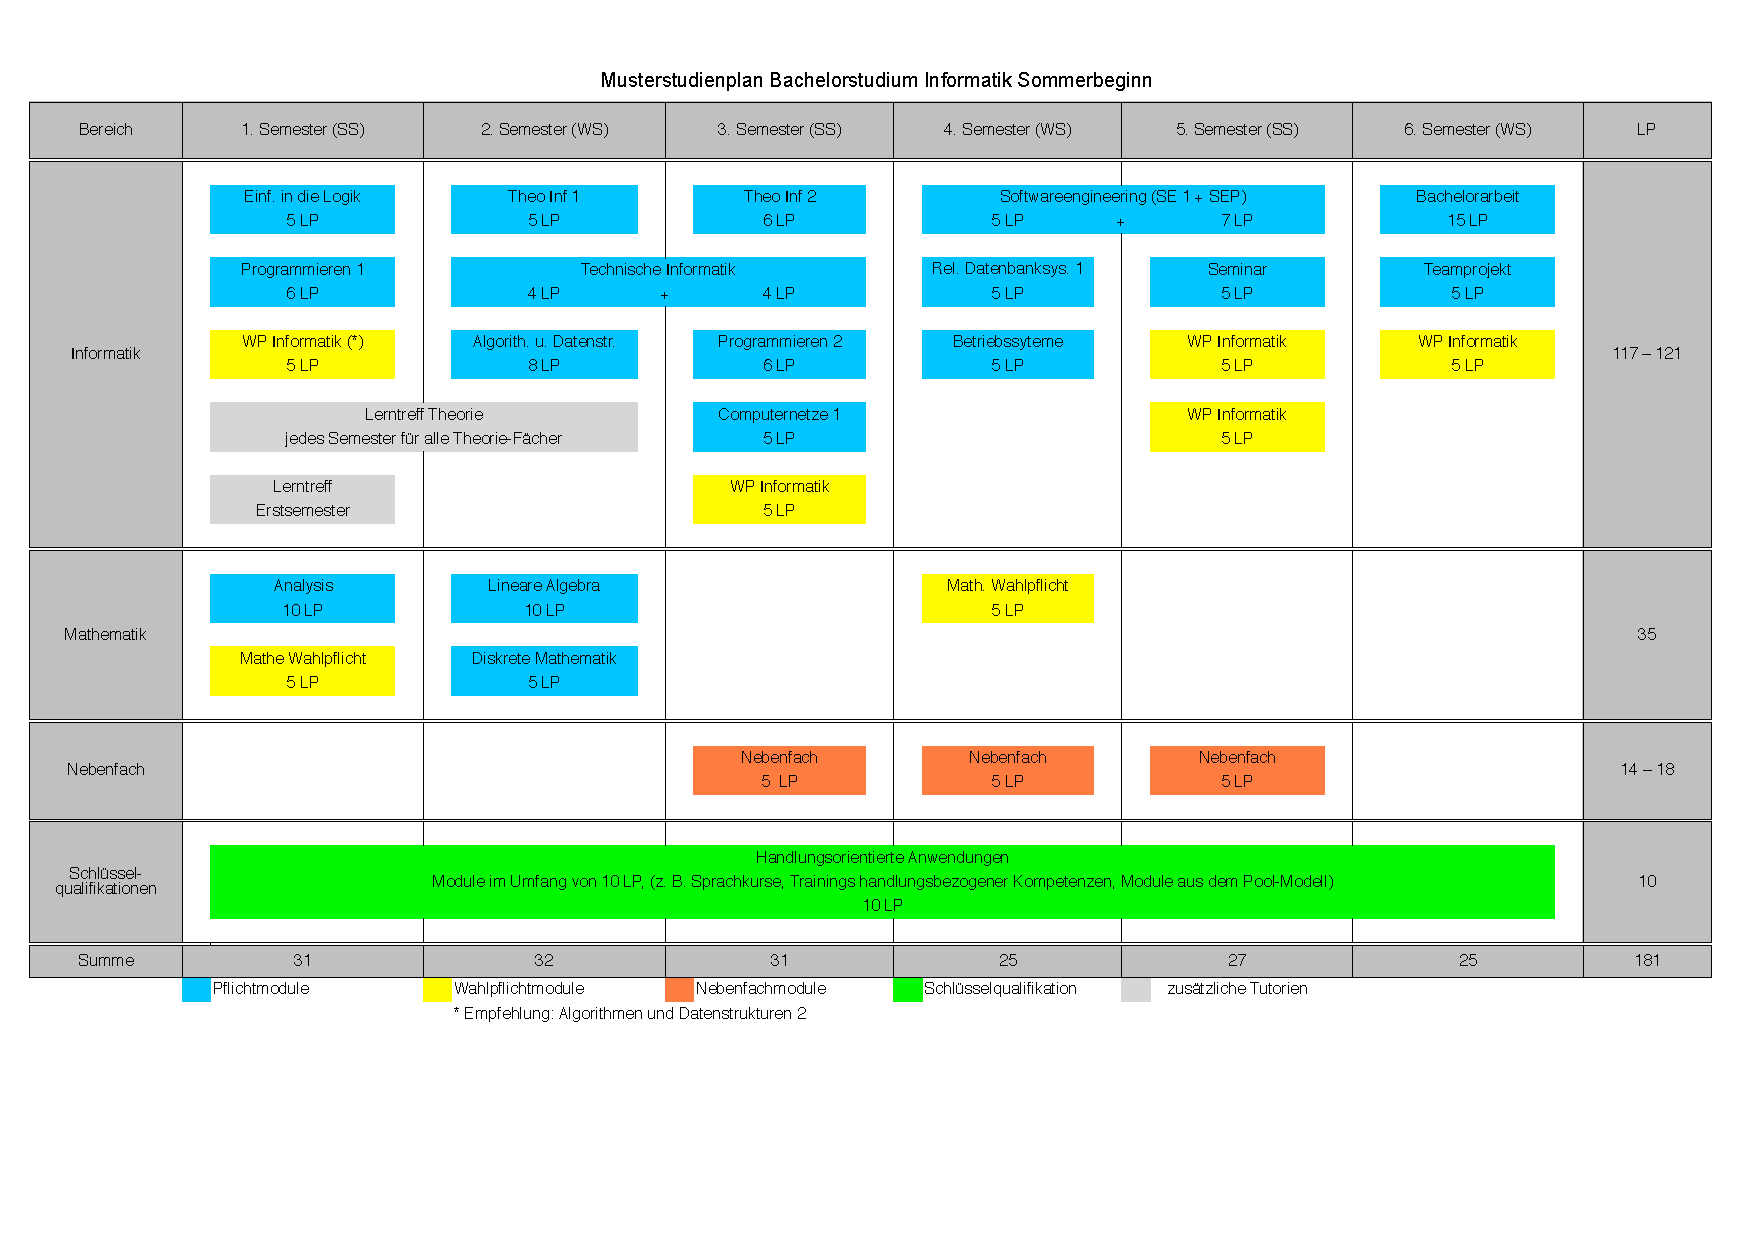
\includegraphics[angle=90, totalheight=\textheight]{bilder/studienplan_bsc_ss/Musterstudienplan_SoSe16.pdf}
	% 	\end{center}  
	% \end{minipage}

	% \begin{minipage}[H]{1.0\linewidth}
	% 	\begin{center}     
	% 	\label{musterstudienplan}
	% 	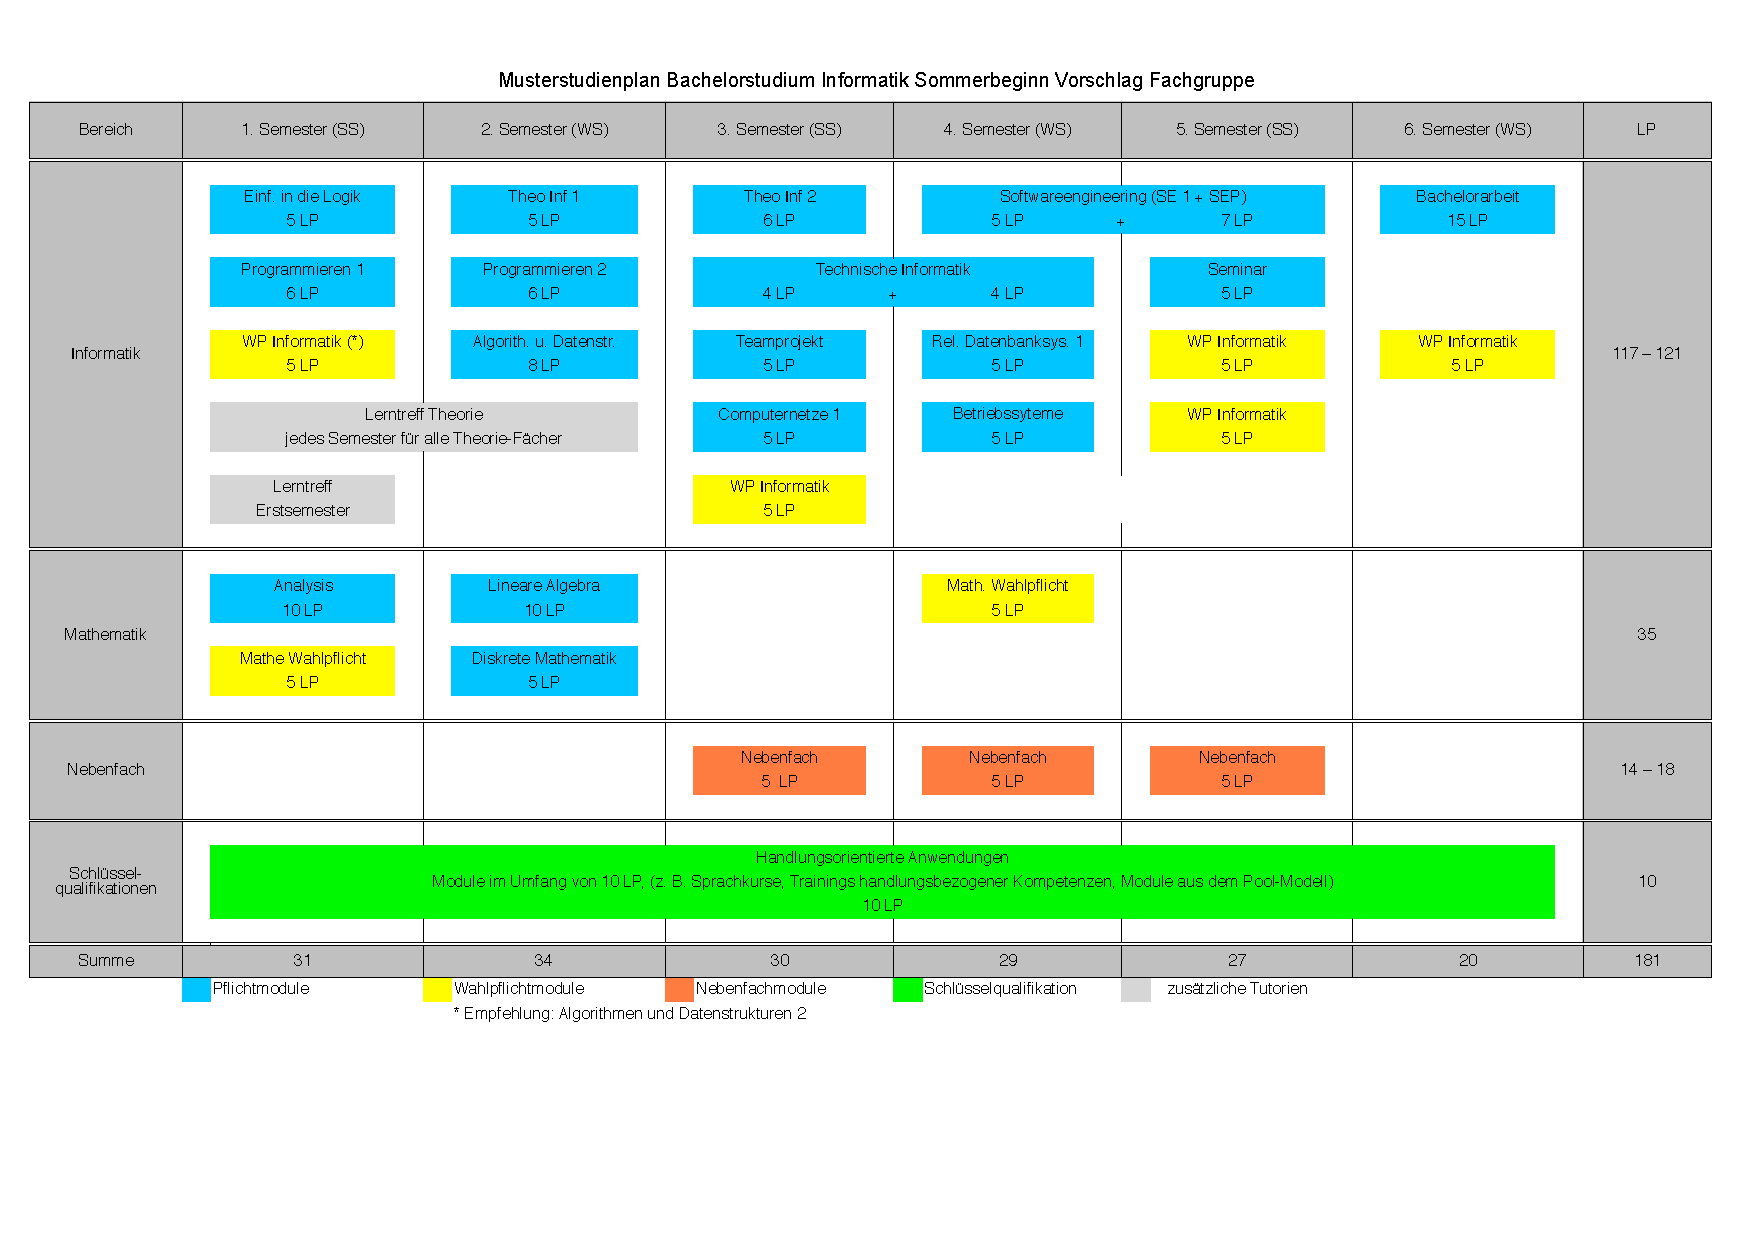
\includegraphics[angle=90, totalheight=\textheight]{bilder/studienplan_bsc_ss/Musterstudienplan_SoSe16_Empfehlung_FG.pdf}
	% 	\end{center}  
	% \end{minipage}
}
